\documentclass[11pt]{article}
\usepackage[a4paper,margin=0mm]{geometry}
\usepackage{fontspec}
\usepackage[french]{babel}
\usepackage{xcolor}
\usepackage{tikz}
\usepackage[most]{tcolorbox}
\usepackage{pdfpages}
\usepackage{hyperref}
\setmainfont{DejaVu Serif}
\setsansfont{DejaVu Sans}
\definecolor{EDBlue}{HTML}{214D6B}
\definecolor{EDGold}{HTML}{F7F1DE}
\definecolor{EDGreen}{HTML}{EDF5EA}
\definecolor{EDPaleBlue}{HTML}{EAF2F7}
\definecolor{EDGrey}{HTML}{6F6F6F}
\pagestyle{empty}

\hypersetup{
  pdftitle={ED-POMDP en clair - Guide de lecture français v1.9},
  pdfauthor={Guillaume Harbonnier},
  pdfsubject={Évolution éditoriale conservatrice de la v1.8 et export de l'ancienne Annexe G}
}
\begin{document}

% Page liminaire ajoutée en v1.9.
\null
\begin{tikzpicture}[remember picture,overlay]
  \node[anchor=north east,text=EDGrey,font=\fontsize{8.5}{10}\selectfont] at ([xshift=-28mm,yshift=-9mm]current page.north east) {ED-POMDP en clair - Guide de lecture français};
  \node[anchor=north,text=EDBlue,font=\bfseries\fontsize{18}{22}\selectfont] at ([yshift=-34mm]current page.north) {Mode d'emploi et glossaire de première lecture};
  \node[anchor=north,fill=EDGold,rounded corners=5mm,text width=150mm,inner xsep=6mm,inner ysep=5mm,align=justify,font=\fontsize{9.3}{10.5}\selectfont] at ([yshift=-65mm]current page.north) {Le guide suit une progression en spirale : la première lecture donne le problème, les paris et les résultats ; les annexes A à F reviennent ensuite sur les formules, les calculs et leurs limites. Les termes ci-dessous sont des repères, pas un cours préalable. Le document companion avancé traite séparément l'estimation d'état, la recherche opérationnelle et l'apprentissage de politiques.};

  \foreach \x/\y/\bg/\title/\body in {
    25/98/EDGreen/{État latent}/{État réel supposé exister mais non observé directement.},
    25/118.5/EDGreen/{Croyance, prior, posterior}/{Distribution de probabilités ; avant observation = prior, après observation = posterior.},
    25/139/EDPaleBlue/{Calibration}/{Accord entre les probabilités annoncées et les fréquences réellement observées.},
    25/159.5/EDGreen/{Score de Brier}/{Erreur quadratique d'une prévision probabiliste binaire : $(p-y)^2$.},
    25/180/EDGreen/{ECE et intervalle (bin)}/{Écart moyen de calibration après regroupement des probabilités proches en intervalles.},
    25/200.5/EDPaleBlue/{Seed}/{Numéro qui permet de reproduire exactement un même scénario aléatoire.},
    25/221/EDGreen/{Cellule et appariement}/{Groupe expérimental ; les politiques sont comparées sur le même scénario, paire par paire.},
    25/241.5/EDGreen/{Baseline}/{Méthode de comparaison plus simple ou différente.},
    25/262/EDPaleBlue/{Endpoint}/{Mesure finale utilisée pour juger un résultat.},
    109/98/EDGreen/{Hypothèse nulle et p-value}/{La p-value mesure la rareté du résultat si l'hypothèse d'équivalence était vraie.},
    109/118.5/EDGreen/{Bootstrap apparié}/{Rééchantillonnage avec remise des mêmes paires pour mesurer la variabilité de l'effet.},
    109/139/EDPaleBlue/{Permutation appariée}/{Échange aléatoire des étiquettes dans chaque paire pour construire une distribution nulle.},
    109/159.5/EDGreen/{Holm}/{Correction progressive qui protège une famille de nombreux tests contre les faux positifs.},
    109/180/EDGreen/{Identifiabilité}/{Possibilité de distinguer les causes cachées à partir des observations disponibles.},
    109/200.5/EDPaleBlue/{Modèle mal spécifié}/{Modèle dont les probabilités supposées ne correspondent pas au monde qui produit les données.},
    109/221/EDGreen/{Cote probabiliste (odds)}/{Rapport $p/(1-p)$, utile pour exprimer une mise à jour bayésienne.},
    109/241.5/EDGreen/{Rapport de vraisemblance}/{Pouvoir d'une observation à favoriser une hypothèse plutôt qu'une autre.},
    109/262/EDPaleBlue/{VOI / EVI}/{Valeur attendue de l'information : gain décisionnel attendu d'une preuve, avant son résultat.}
  }{
    \node[anchor=north west,fill=\bg,rounded corners=3mm,minimum width=76mm,minimum height=17mm,text width=68mm,inner xsep=4mm,inner ysep=2.4mm,align=left] at ([xshift=\x mm,yshift=-\y mm]current page.north west) {\textcolor{EDBlue}{\bfseries\fontsize{7.3}{8}\selectfont \title}\\[-0.2mm]{\fontsize{6.4}{7.1}\selectfont \body}};
  }
  \node[anchor=south,text=EDGrey,font=\fontsize{6.5}{7.5}\selectfont,align=center] at ([yshift=6mm]current page.south) {Les noms de fichiers, clés de configuration et identifiants du dépôt restent en anglais lorsqu'ils sont des artefacts techniques.\\Page liminaire non numérotée - Guide principal v1.9};
\end{tikzpicture}
\newpage

% Couverture v1.8 reprise avec deux corrections éditoriales locales.
\includepdf[
  pages=1,
  fitpaper=true,
  pagecommand={
    \begin{tikzpicture}[remember picture,overlay]
      \fill[white] ([xshift=37mm,yshift=-76mm]current page.north west) rectangle ([xshift=-37mm,yshift=-85mm]current page.north east);
      \node[font=\fontsize{8.8}{10}\selectfont] at ([yshift=-80mm]current page.north) {Guide pédagogique français - Document compagnon - Version 1.9};
      \fill[white] ([xshift=14mm,yshift=-90mm]current page.north west) rectangle ([xshift=-14mm,yshift=-153mm]current page.north east);
      \begin{scope}[shift={([xshift=16mm,yshift=-94mm]current page.north west)}]
        \fill[EDGold] (0,0) rectangle (179mm,-47mm);
        \draw[EDBlue!60,line width=.35pt] (0,0) rectangle (179mm,-47mm);
        \node[anchor=north west,text width=167mm,font=\bfseries\fontsize{9.3}{11}\selectfont] at (4mm,-4mm) {À lire avant le papier scientifique};
        \node[anchor=north west,text width=167mm,align=justify,font=\fontsize{8.3}{9.4}\selectfont] at (4mm,-10mm) {Le rapport Step 2 Benchmark Close-Out est une conclusion scientifique et un document d'audit. Le présent guide explique le problème, la genèse de l'approche, l'intuition, les deux paris scientifiques, leur tentative de falsification et le sens des résultats. Les annexes A à F approfondissent la contestation du modèle, sa généalogie, la mesurabilité des variables, les données synthétiques, le fonctionnement du code et la mécanique statistique utilisée pour juger un résultat. Certaines notions sont d'abord introduites par leur rôle, puis expliquées et calculées dans les annexes : une seconde lecture est volontairement utile. L'ancienne Annexe G est publiée séparément comme document companion avancé. Le guide ne remplace pas les artefacts formels et ne modifie aucun claim.};
      \end{scope}
    \end{tikzpicture}
  }
]{base/ED_POMDP_En_Clair_FR_v1.8.pdf}

% Pages héritées inchangées : v1.8 pages 2 à 30.
\includepdf[pages=2-30,fitpaper=true,pagecommand={}]{base/ED_POMDP_En_Clair_FR_v1.8.pdf}
\end{document}
